%SOP Template 



\documentclass[12pt]{../SOP4_alpha}\usepackage[]{graphicx}\usepackage[]{xcolor}
% maxwidth is the original width if it is less than linewidth
% otherwise use linewidth (to make sure the graphics do not exceed the margin)
\makeatletter
\def\maxwidth{ %
  \ifdim\Gin@nat@width>\linewidth
    \linewidth
  \else
    \Gin@nat@width
  \fi
}
\makeatother

\definecolor{fgcolor}{rgb}{0.345, 0.345, 0.345}
\newcommand{\hlnum}[1]{\textcolor[rgb]{0.686,0.059,0.569}{#1}}%
\newcommand{\hlsng}[1]{\textcolor[rgb]{0.192,0.494,0.8}{#1}}%
\newcommand{\hlcom}[1]{\textcolor[rgb]{0.678,0.584,0.686}{\textit{#1}}}%
\newcommand{\hlopt}[1]{\textcolor[rgb]{0,0,0}{#1}}%
\newcommand{\hldef}[1]{\textcolor[rgb]{0.345,0.345,0.345}{#1}}%
\newcommand{\hlkwa}[1]{\textcolor[rgb]{0.161,0.373,0.58}{\textbf{#1}}}%
\newcommand{\hlkwb}[1]{\textcolor[rgb]{0.69,0.353,0.396}{#1}}%
\newcommand{\hlkwc}[1]{\textcolor[rgb]{0.333,0.667,0.333}{#1}}%
\newcommand{\hlkwd}[1]{\textcolor[rgb]{0.737,0.353,0.396}{\textbf{#1}}}%
\let\hlipl\hlkwb

\usepackage{framed}
\makeatletter
\newenvironment{kframe}{%
 \def\at@end@of@kframe{}%
 \ifinner\ifhmode%
  \def\at@end@of@kframe{\end{minipage}}%
  \begin{minipage}{\columnwidth}%
 \fi\fi%
 \def\FrameCommand##1{\hskip\@totalleftmargin \hskip-\fboxsep
 \colorbox{shadecolor}{##1}\hskip-\fboxsep
     % There is no \\@totalrightmargin, so:
     \hskip-\linewidth \hskip-\@totalleftmargin \hskip\columnwidth}%
 \MakeFramed {\advance\hsize-\width
   \@totalleftmargin\z@ \linewidth\hsize
   \@setminipage}}%
 {\par\unskip\endMakeFramed%
 \at@end@of@kframe}
\makeatother

\definecolor{shadecolor}{rgb}{.97, .97, .97}
\definecolor{messagecolor}{rgb}{0, 0, 0}
\definecolor{warningcolor}{rgb}{1, 0, 1}
\definecolor{errorcolor}{rgb}{1, 0, 0}
\newenvironment{knitrout}{}{} % an empty environment to be redefined in TeX

\usepackage{alltt}

\usepackage[english]{babel}
%\usepackage{blindtext}
%\usepackage{lipsum}

%\usepackage[version=4]{mhchem} 
\usepackage{pdfpages}

\title{Soil Loss on Ignition}
\date{7/12/2015}
\author{Ever Cook}
\approved{Los Huertos}
\ReviseDate{\today}
\SOPno{32 v0.1}
\IfFileExists{upquote.sty}{\usepackage{upquote}}{}
\begin{document}
\SweaveOpts{concordance=TRUE}

\maketitle

\section{Scope and Application}

\NP Loss on Ignition (LOI) is used to determine organic matter content (OM\%) in soil samples. This is important for indirectly estimating soil organic carbon (SOC) in agricultural topsoil. 

\NP The applications implement SFU Soil Science Lab method (Robertson, 2011) *and add Aaron's method paper for temperature*.

\section{Summary of Method}

\NP This method will cover how to conduct a LOI procedure in the Pomona College Geology Department Lab. Ignition of the soil samples in a muffled furnace burns off any organic matter, leaving only the mineral content. The weight difference of the samples before and after ignition represents the OM\%. This method uses a temperature of 360^\circ$C for 2 hours.

\tableofcontents

\newpage

%\section{Acknowledgements}

%\section{Definitions}

%\NP Crucible


\section{Biases and Interferences}

\NP The following are parameters that might influence the results of the LOI test and thus, we review methods that would best fit the type of soils from our samples.

\begin{description}
  	\item[Clay content] Soil texture has many influences, two of which being climate and parent material 
		\item [Ignition temperature] If the temperature is not hot enough, there may be OM remaining in the samples after ignition.
		\item [Ignition duration] If the samples are not burned for long enough, there may be OM remaining in the samples after ignition.
\end{description}


\section{Health and Safety}

\NP The muffled furnace burns up to 3000$^\circ$C, posing a significant threat to 4th degree burns if precautions aren't taken.

\subsection*{Safety and Personnnel Protective Equipment}

\NP Care should be taken to prevent burns. Remove crucibles from the furnace with tongs and heat-proof gloves. Wait at least 1 hour for them to cool down before handling with bare hands. In case of contact, run skin under cold water for 15 minutes and follow lab procedures for emergency. 

\section{Personnel \& Training Responsibilities}

\NP Researchers training is required before the procedures in this method can be used.

\NP Researchers using this SOP should be trained for the following SOPs:

\begin{itemize}
  \item SOP01 Laboratory Safety
  \item SOP07 Using Balances
  \item SOP15 Using Drying Ovens
\end{itemize}

\newpage 

\section{Required Materials and Apparati}

\begin{enumerate*}
	\item Porcelain crucibles
	\item Soil samples
	\item Muffled furnace
	\item Drying oven
	\item Tongs
	\item Heat-proof gloves
	\item Jack stand
	\item Metal tin
	\item Scoopula
	\item Combustion residue mapping sheet
\end{enumerate*}

\section{Reagents and Standards}

%\begin{enumerate*}
%	\item 
%\end{enumerate*}

\section{Estimated Time}

\NP This procedure requires several days to complete.

%\begin{table}
%\begin{tabular}{llll}\hline
%Task          & Time          & Elapsed Time  & Time until completion \\ \hline\hline
%Collect Soil  & 1-3 hours     & 1-3 hours     &         \\ \hline
%\end{tabular}
%\end{table}

\section{Sample Collection, Preservation, and Storage}



\section{Procedure}

\subsection{Preperation}

\NP Prepare the soil samples in advance in the EA lab. Samples may be sieved with a 2mm sieve.
  The following steps use a drying oven to remove moisture content from the soil and the crucibles that may affect the true dry weights. You can collect soil \% moisture data while simultaneously prepping for LOI.
  
  \begin{enumerate}
	  \item Weigh and record the weight of a labeled metal tin. Add about 3 scoops fo soil using the scoopula into the tin. Record the soil ID, tin #, tin weight, and soil 'wet' mass.
	  \item Oven-dry tins at 105$^\circ$C for 24 hours.
	  \item Once done, open the oven door for about 15 min to cool down. Take samples out of the oven once cool to touch. Weigh and record weigh
	  \item Oven-dry crucibles in the same manner. %Weigh and record crucible weight on the Combustion residue mapping sheet
	\end{enumerate}
	
\subsection{Ignition}

\NP Once ready for ignition, head to the Geo Lab. If the oven is not on already, we can begin heating the oven while preparing the crucibles. Ask the lab technician for help if needed. The Geology Dept. has multiple muffled furnaces. This SOP instructs how to use the Nabertherm furnace 

\NP We will load the furnace while hot and keep it on continuously and overnight until finished with all samples. Frequent reheating can harm the heating coils.

\NP Use the dial knob to set the furnace to the correct program preset called "LOI" and assure it is set to the correct temperature of 360^\circ$C. Press the start button. The LCD screen will tell you the current temperature inside the furnace.

%image

\NP Then, for each sample...
  \begin{enumerate}
	\item Record the weight of the crucible on a scale capable of precision to 0.0001. It may have an assigned #, if not write one with Sharpie on the side of the crucible.
	\item Add oven-dried sample into the crucible.
	\item Weigh and record this as the pre-ignition weight. 
		\end{enumerate}
		
\NP As you prepare the crucibles, use the Combustion Residue Mapping Sheet to map to lay out where you'll put each crucible in the furnace. 8 crucibles can fit in the furnace.
\NP This is important to prevent mixing up samples. Permanent marker will leave a light stain, but shouldn't be relied on. Use the hole on the plate to help you determine direction.

% image here
 
\NP Arrange the crucibles in order on the furnace plate atop the jack stand. The jack stand should be level with the inside of the furnace for easy loading.

\NP Once the furnace is ready, use the tongs and heat-proof gloves push the furnace plate in like so.

% Put image in

\NP Set a timer for 2 hours.

\NP Find something to do in the meantime like prepping the next batch of crucibles.
  
  
  ---------
  
  

\subsection{Determining Proportion of Soil Passing No. 10 Sieve}

\NP Soils are defined as particles that are less than 2 mm. Thus, we begin by removing the gravel, particles that exceed the sand-sized particles, >2.0 mm. These particles, however, influence the soil texture, so we will quantify the contribution of particles that exceed 2 mm. 

\NP We can do this by analyzing the soil that can pass through the No. 10 sieve, which has a mesh size of 2 mm.  

  
\subsection{Measuring and Correcting for Soil Water Content}

\NP We will use air-dried soil for our test. However, even air-dried soil contains water. This moisture is associated with clay particles, salts, and organic matter and is often referred to as hygroscopic water. To calculate the soil moisture content, we weigh the soil before and after oven drying the soil at 110$^\circ$ C. Once we determine the moisture content, we can use the moisture content to correct for the water in the air-dried soil. Because this method relies on the change in soil mass, the water content is often referred to as gravimeter water content as opposed to a volumetric water content.

\NP This temperature is somewhat arbitrary, and clay minerals in particular may contain 10-15\% water (dry basis) at 400$^\circ$ C (Gardner 1986).  As temperature increases, first water in soil pores evaporates, then water adsorbed to mineral surfaces, followed by water between lattice layers and that which forms part of the mineral lattice itself.  The exact quantities and patterns of release in a hetergeneous mixture like soil depends on the particular mix of minerals making up a sample.  Water adsorbed to organic components (as well as other volatile organic substances) will also evaporate over a range of temperatures.  The key point is to specify the temperature used when reporting moisture data.

\NP To determine the hygroscopic water content,

\begin{enumerate}
	\item Weigh and record the weight of a soil tin (Appendix A, Box 13) and the tin \# (Appendix A, Box 12);
	\item Remove a 10-15 gram sub-sample from the air-dried soil that passed through the No. 10 sieve, put the sub-sample into the pre-weighed soil tin and record the weight (Appendix, Box 14);
	\item Dry the sample in a drying oven set at 110 $^\circ$ C for approximately 24 hours;
	\item Allow the tins to cool and record the oven-dried weight (Appendix, Box 15). 
\end{enumerate}

\NP We calculate the  hygroscopic moisture content we subtract the mass of oven-dried sample and the air-dried mass before drying, usually less than one, unless there is no hygroscopic moisture, then is is one. Use the following equation to calculate the water content

\begin{equation}
\texttt{Moisture}_H = (\texttt{air-dry mass w/tin} - \texttt{oven-dried mass w/tin})/(\texttt{air-dried mass} - \texttt{tin mass})
\end{equation}

\noindent $Moisture_H$ can be calculated using R code developed for this SOP. See Appendix B for a user guide for the program. 

\subsection{Calculating Soil Sample Mass}

\NP We then calculate the ``Total Sample Represented'' in the hydrometer test as the mass of soil in hydrometer test as the oven dry mass used by the percent passed through 2 mm sieve and multiply by 100.

\NP We will analyze air dried soil -- that has passed through a No. 10 sieve. 

\begin{equation}
W = oven dry mass * percent passing 2mm sieve * 100
\end{equation}

\begin{equation}
WB = \frac{M_{air}*10000}{Per_{No.10} * (100 + Moisture_H)}
\end{equation}

\NP But since the sample has hygroscopic water, we will use the correction factor above to weigh a ``oven-dried equivalent'', $DW_e$. 

\NP If the soils are coarse textured (>70\% sand), will will use $DW_e$ of 100 g, otherwise 50 g is sufficient.

\NP Since air dried soil contains water, the soil sample used will weigh slightly more than 50g or 100 g for sandy soils where $DW_e = DW_{air} * (1 + DW_c)$,\footnote{I need to check this!}, thus we can re-arrange the equation to determine the amount of air-dried soil to use for our test:

\begin{equation}
DW_{air} = 50/(1+DW_c)
\end{equation}

\noindent and for sandy soils,

\begin{equation}
DW_{air} = 100/(1+DW_c)
\end{equation}



--------


		\begin{table}
		\begin{tabular}{lrrr}\hline
Obs. & Soil Reading Times 		& Temperture		& Blank Hydrometer \\ \hline\hline	
0		& Before Inverting (0 seconds)		&	 X	&		X		\\
1		& 40 seconds (Repeat twice) 			&	 		&			  \\
2		&	2.0 minutes 										&			&       \\
3		&	5.0 minutes 										&	 X 	&		X   \\
4		&	15 minutes 											&	 		&   	  \\
5	 	& 30 minutes 											&			&				\\
6		& 60 minutes 											&		X	& 	X		\\
%X		& 90 minutes 										&			&				\\
7		& 2	hours													& 	X	& 	X		\\
8		& 3 hours (optional)							&		X	& 	X		\\
9   & 6 or 8 hours (optional)					&		X	& 	X		\\
10		& 24 hours											&		X	&  	X 	\\\hline		
		\end{tabular}
		\caption{Reading times modified from \textbf{citet{standard2007d422}}. These times can be adjusted, be sure to record the actual times in Boxes 19 and 20.}
		\label{tab:ReadingTimes}
	\end{table}
	
	\item Be sure that the cylinder is back from the edge of the counter and in a location where it won't be disturbed.	
	
\end{enumerate}

\subsection*{Determining Proportion of Soil Retained No. 200 Sieve}

\NP Particles retained on the No. 200 sieve are larger are often categorized as sand. As the hydrometer does very little to distinshin between size fractionation of sand -- very fine, fine, medium, course, and very course sand. 

\NP But collecting the particles on the No. 200 sieve, we can use seives to better understand the soil characteristics. We can do this by analyzing the mass of the soils retained on the No. 200 sieve, which has a mesh size of XX 0.125 mm.  

\begin{enumerate}
	\item Poor the contents of the cylinder through a No. 200 sieve;
	\item Using the sink with a sediment trap, wash the soil in the sieve until the water leaving the sieve is clear. 
	\item Select a soil tin, and record the tin \# (Box XX) and tin mass (Box XX). 
	\item Carefully wash the soil from the tin into the soil, without damaging the sieve screen. The screens are quite delicate, so using a squeeze bottle is probably best. Using a brush or metal device will force particles into the screen, which can get stuck, distort and stretch the mesh openings or otherwise damage them. 
	\item Weigh the dry soil with the soil tin and record the results in Box Xx.
\end{enumerate}

\section{Recording the Results}

Record the results in Appendix A, Then enter the data into the data entry form (\href{test}{http\\:test}. Other columns calculations will be produced with the R code from Appendix B.  

Do not put commas in text fields -- if you do the download... it will create extra columns and the data will be misaligned.

\section{Data Analysis and Calculations}

Once the data has been entered in the online form, you can extract the data as a csv file. This csv file can then be called by R to calculate the data automatically, using the following functions. 

\subsection*{Importing Data}

Import and check data integrity

\begin{knitrout}
\definecolor{shadecolor}{rgb}{0.969, 0.969, 0.969}\color{fgcolor}\begin{kframe}
\begin{alltt}
\hlcom{#hydrometer = import()}
\hlcom{#head(hydrometer)}
\hlcom{#str(hydrometer)}
\end{alltt}
\end{kframe}
\end{knitrout}

What should you be looking for?  We want to make sure the data shown are the same as expected. There are several ways to look at the data to determine this. I have shown two ways. 1) Looking at the header (first six observations), then we evaluate the structure of the dataframe.
 
\subsection{Calculating effective diameter, $D_e$}


\subsection{Calculating the Percent Finer, PF}


\subsection{Graphing and Interpreting the Results}

\section{QC/QA Criteria}

\section{References}

\NP D422...

\NP Wilde, S.A., R.B. Corey, J.G. Iyer, and G.K. Voigt.  1979.  Soil and Plant Analysis for Tree Culture.  Oxford and IBH Publishing Co., New Delhi.  Pp. 12-13.

\NP Anderson, J.M., and J.S. Ingram, eds.  1993.  Tropical Soil Biology and Fertility:  A Handbook of Methods. 2nd ed.  CAB International, Wallingford, UK.  P. 93-94.

\section{Appendix A. Data Sheet}

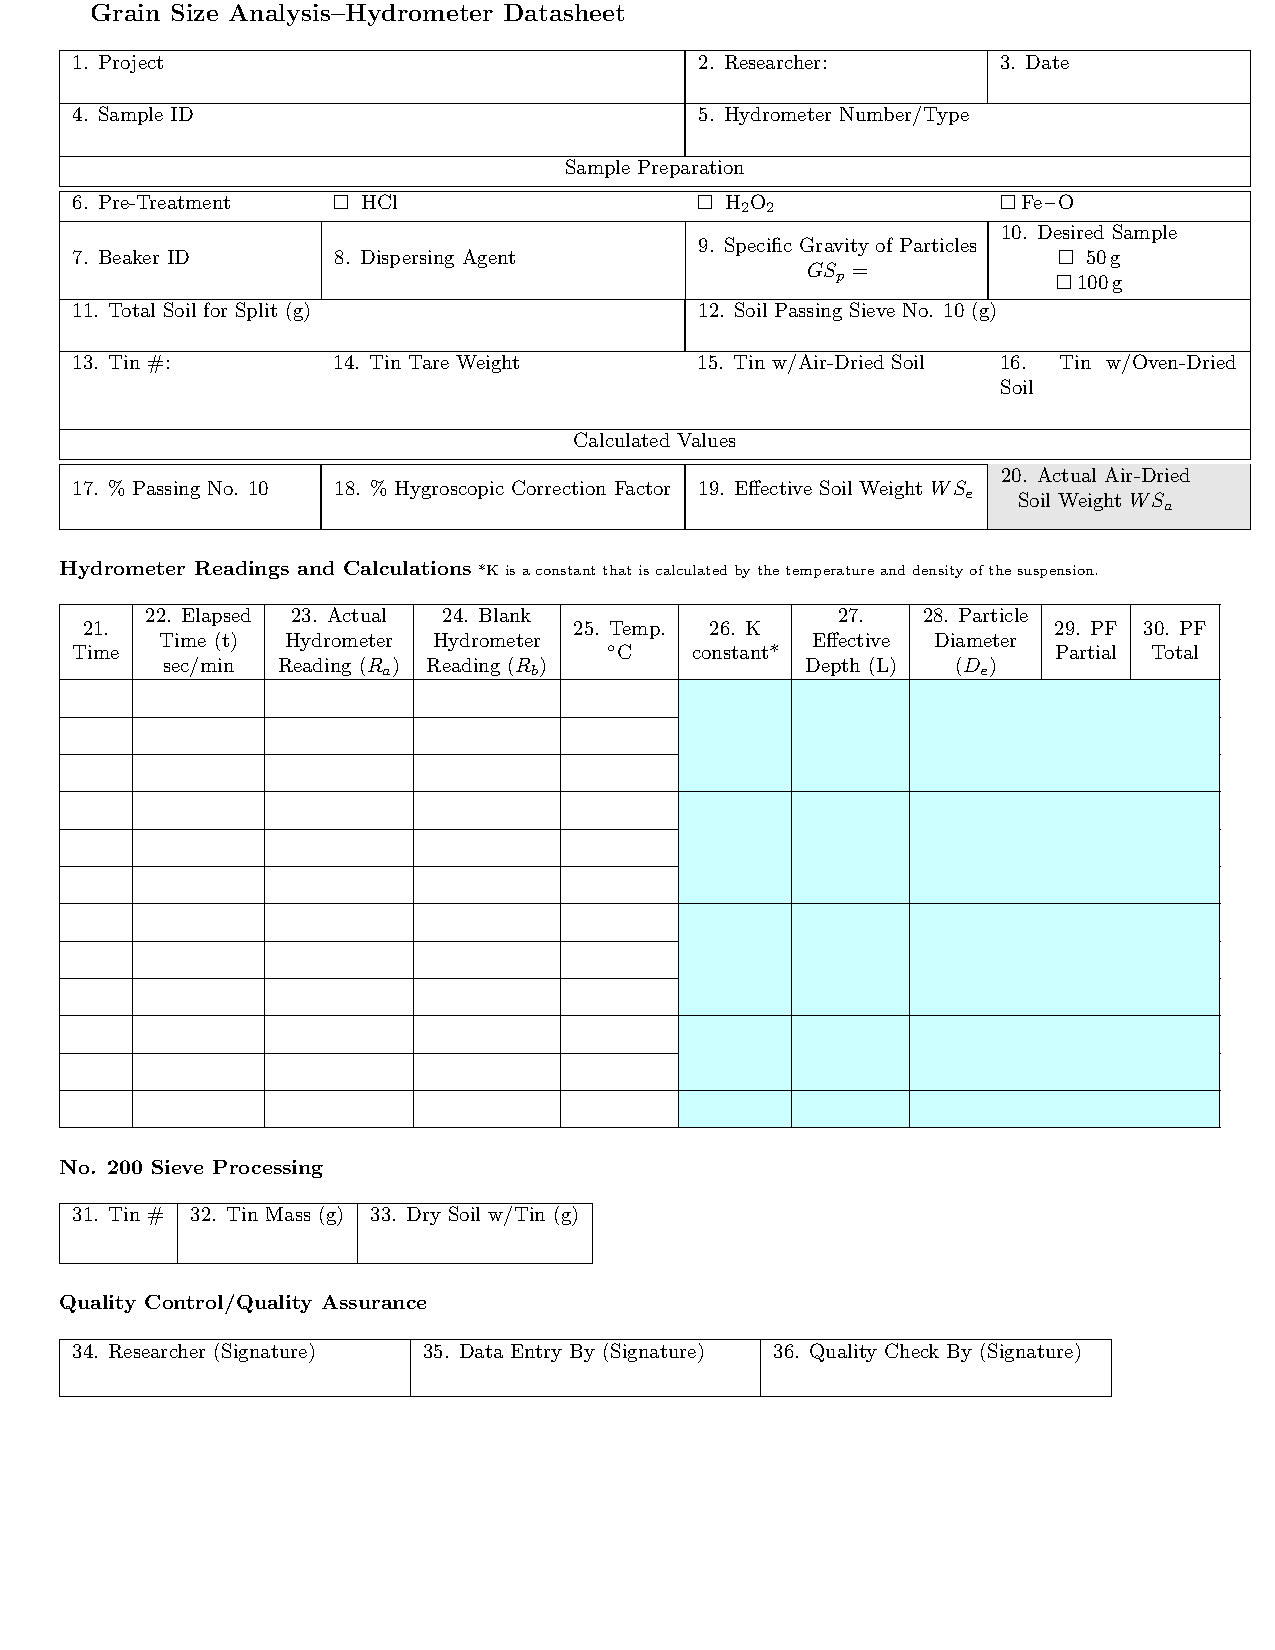
\includepdf[pages=-]{DataSheetv3}


\newpage
\section{Appendix B: R code to calculate parameters for the SOP}

% \input{Appendix B}	

\end{document}
